\chapter{Evaluation and Experiments}

This chapter describes the evaluation methodology and outlines the metrics and figures that we used to quantify the performance of our learned policies on both single-quadrotor and multi-quadrotor cable-suspended payload transport tasks.

\section{Experimental Setup}
We first evaluate the performance of our learned policies in our simulation environment. We use only the actor network for evaluation, as the critic is not needed. The policies are trained using the \gls{ippo} algorithm.
All experiments were conducted in simulation using a policy frequency of 250 Hz with one physics step per control action. We set both observation and actuator noise to zero, randomized thrust within 80-100\% thrust range, used a 0.3 m cable length, and fixed the payload mass at 0.01 kg. 

Two primary tasks were evaluated: 
 recovery-from-harsh-conditions task and figure-eight trajectory tracking task. The recovery task involved stabilizing the payload at a target position after being disturbed, while the trajectory tracking task required the quadrotor to follow a precomputed figure-eight path while keeping the payload stable.

In the recovery task, episodes lasted 2,500 steps, the payload target remained fixed at $(0 0 1.5)$ m, and the agent began from random harsh initial states. The payload and quadrotor position aswell as the quadrotors orientation and velocity are randomized.
 metrics were gathered over 1,000 rollouts. We evaluate the specific policies for single quad with payload, teams of two, three, and five quadrotors were evaluated, each initialized as described in section X\todo{ref}. The payload was always initialized at $(0 0 1.5)$ m, and the quadrotors were positioned randomly in a half-sphere around it. Its importent to not that this includes differnt cable modes, with sometimes the cable being slack and sometimes taut. Forcing the quadrotor to stabilize the payload in all modes. These states emulate the state after a strong disturbance, like a collision with an obstacle or the quadrotors being thrown into the air.

In the figure-eight tracking task, each episode ran for 5,000 steps simulating 20s, the payload has to follow a precomputed figure-eight path, and the quadrotor always initialized at the center with quads in random positions, with performance aggregated over 100 rollouts. 


\section{Single-Quadrotor Payload Control}
We first evaluate the learned policy on the single-vehicle case, testing both harsh condition recovery and trajectory tracking on a figure-eight path. We run each of them with the a ploicy trained specifically for the single quadrotor with payload scenario. The results are shown in Figure \ref{fig:payload_error_over_time_single} and Figure \ref{fig:one_recovery}.
Figure \ref{fig:one_recovery} shows some example runs of the recovery task, where the quadrotor is initialized in random states and has to stabilize the payload at the target position $(0 0 1.5)$ m. The quadrotor successfully stabilizes the payload within 2 seconds for most initial conditions. In the figure the bottom two runs labeled 6 and 7 show takeoff from the ground, which is hard due to a very sudden mode switch from slack to taut cable close to the ground. Runs 1 to 5 show the active swing counteraction of the quadrotor, where it actively stabilizes the payload on the path to the target. Runs 3 and 4 specifically show a very strong initial payload swing. All runs stabilize the payload swing before reaching the target posistion without any oscillations or overshoot. They then stabalize there without much movement for the rest of the run. We can see that the policy generalizes to all relative positions of the payload to the target and the quadrotor to the payload. During recovery the payload reaches speeds of up to 1.7m/s, highlighting the learned agility of the policy. If this level of agility is not desired the speed can be reduced by adjusting the linear velocity components of the reward function.
We here only show recovery from up to 1.5m. This though generalizes to any distance by clipping the length of the position error vector to 1m. 
Additionaly to the qualitative analysis we also show a more thorough statistical analysis in Figure \ref{fig:payload_error_over_time_single}. Here we statisitcally evaluate 1000 recovery runs from harsh conditions. The termination histogram shows that 99\% of harsh inital conditions are recovered successfully, while the remaining terminate right in the beginning due to very harsh initialization. The position error over time also shows that we recover from distances of up to 1m in roughly 2s. It also shows that all runs stabily hove at the target for over 5s after they reaching it.

To show that the position tracking capabilities generalize to a moving setpoint we evaluate on a precomputed figure eight trajectory. For each timestep we sample the policy position setpoint on the figure eight trajectory leading to the tracking behavior shown in figure \ref{fig:one_eight}. The figure shows the path of 5 runs randomly initialized around the start point of the trajectory, with the quads in suboptimal states. The figure shows how the quads very fast manage to stabilize themselfs and then continue after around 3s to very acurately follow the trajectory. Eventhough all quads are initialized with slightly different thrust ranges they all manage to accurately track the correct height of the trajectory.
Due to the policy currently just being able to do position tracking it always slightly lags behind from the trajectory. This can be seen at the end of the trajectory where it does not fully reach the center. This could be reduced by explicitly training on trajectory following and adding multiple trajectory points or velocity states as shown in previous work.

These experiments show that the trained policy for the singel quadrotor with payload case exhibits great payload swing stabilization ability, while also being agile and very accurate in tracking.


\begin{figure}[]
    \centering
    \begin{subfigure}[b]{0.49\textwidth}
        \centering
        
        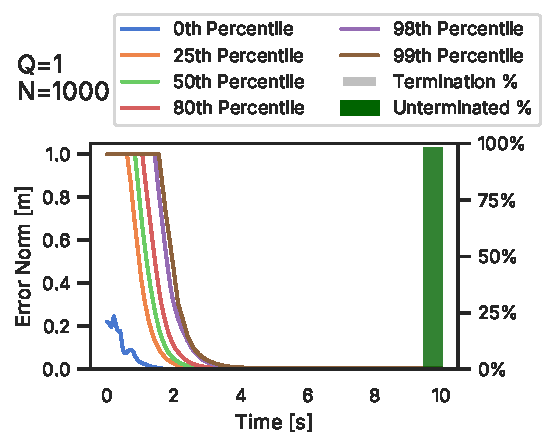
\includegraphics[width=\textwidth]{experiments/one_recovery_error.pdf}
        \caption{Recovery in the single quadrotor with payload scenario from 1000 different initial harsh states. The Percentiles show smooth reduction of the initial high tracking error converging to 0. The termination percentatge shows that most runs are successful and not terminated.}
        \label{fig:payload_error_over_time_single}
    \end{subfigure}
    \hfill
     \begin{subfigure}[b]{0.49\textwidth}
        \centering
        
        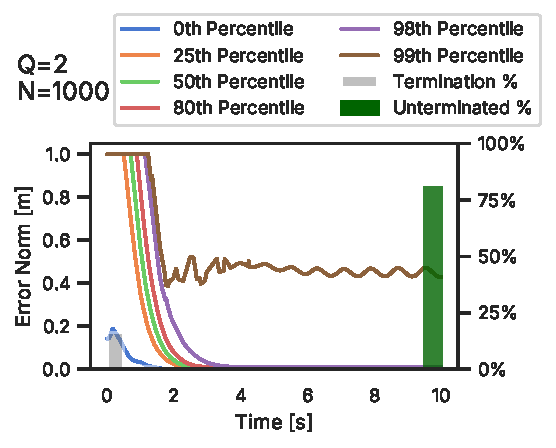
\includegraphics[width=\textwidth]{experiments/two_recovery_error.pdf}
        \caption{Recovery in the two quadrotor with payload scenario from 1000 different initial harsh states. The Percentiles show smooth reduction of the initial high tracking error for most inital harsh states evantually converging to 0. The termination percentage shows that a high number of runs are successful and not terminated while most terminations occur right at initialization, because of very harsh initialization.}
        \label{fig:payload_error_over_time_two}
    \end{subfigure}
    \caption{Performance of a single quadrotor carrying a suspended payload: disturbance recovery and trajectory tracking.}
    \label{fig:single_quad_payload_subfigs}
\end{figure}



\begin{figure}[ht]
    \centering
    
    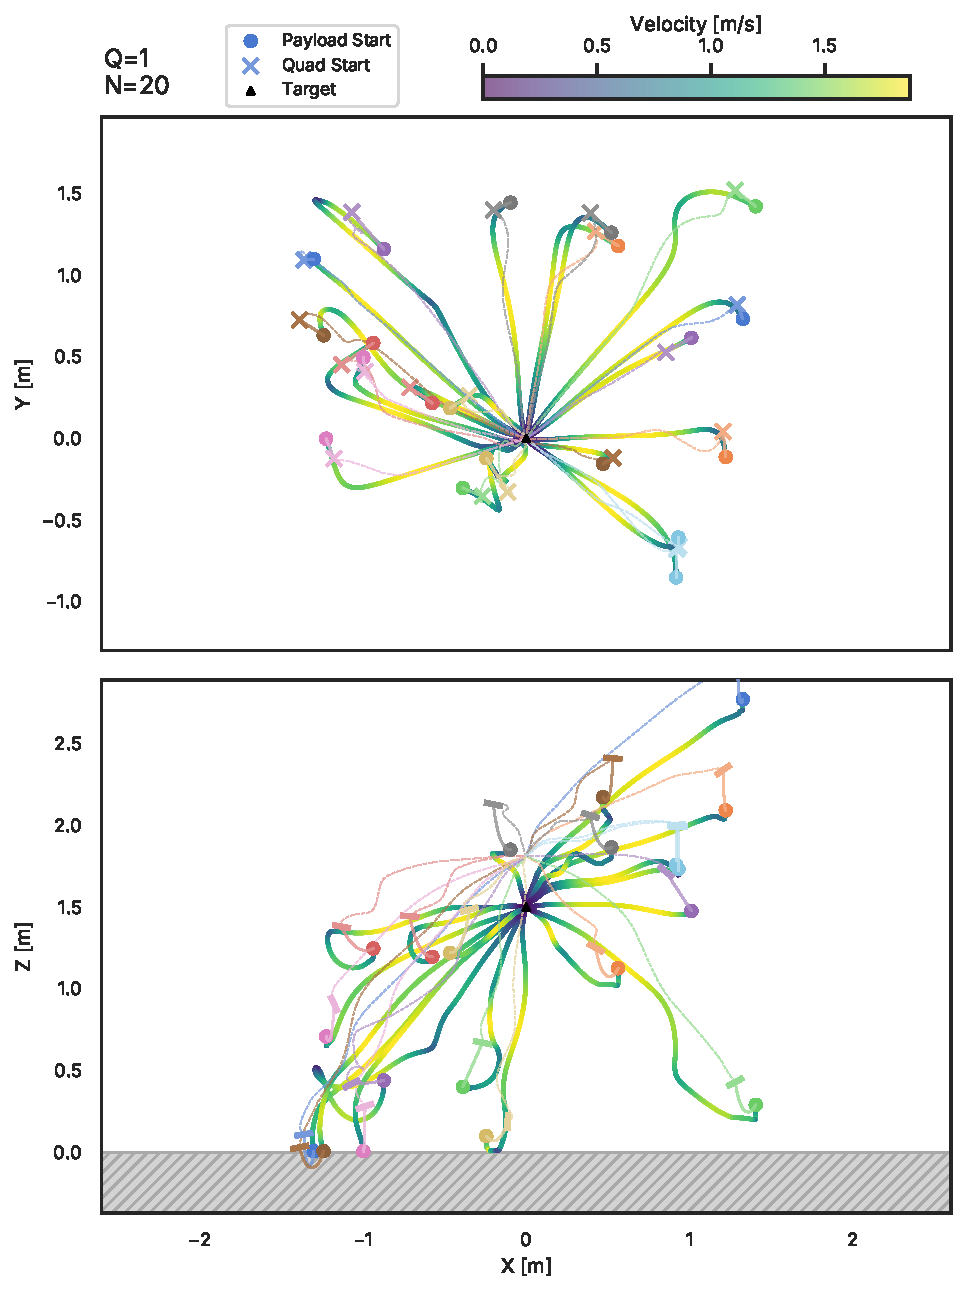
\includegraphics[width=\textwidth]{experiments/one_recovery.pdf}
    \caption{Recovery of one quadrotor with payload from harsh conditions. The top plot is top-down  (xy) view, while the bottom one is side view (xz).
    The figure shows N=8 runs. The position is initialized randomly and the goal is to recover to the target and stabilize. The quadrotor successfully stabilizes the payload within 2 seconds. The initial states of the quadrotor and payload are marked and labeled with their run id. The cables are drawn to represent their mode and cable lengt, slackness in the cable being shown as a curve.}
    \label{fig:one_recovery}
\end{figure}
\begin{figure}[ht]
    \centering
    
    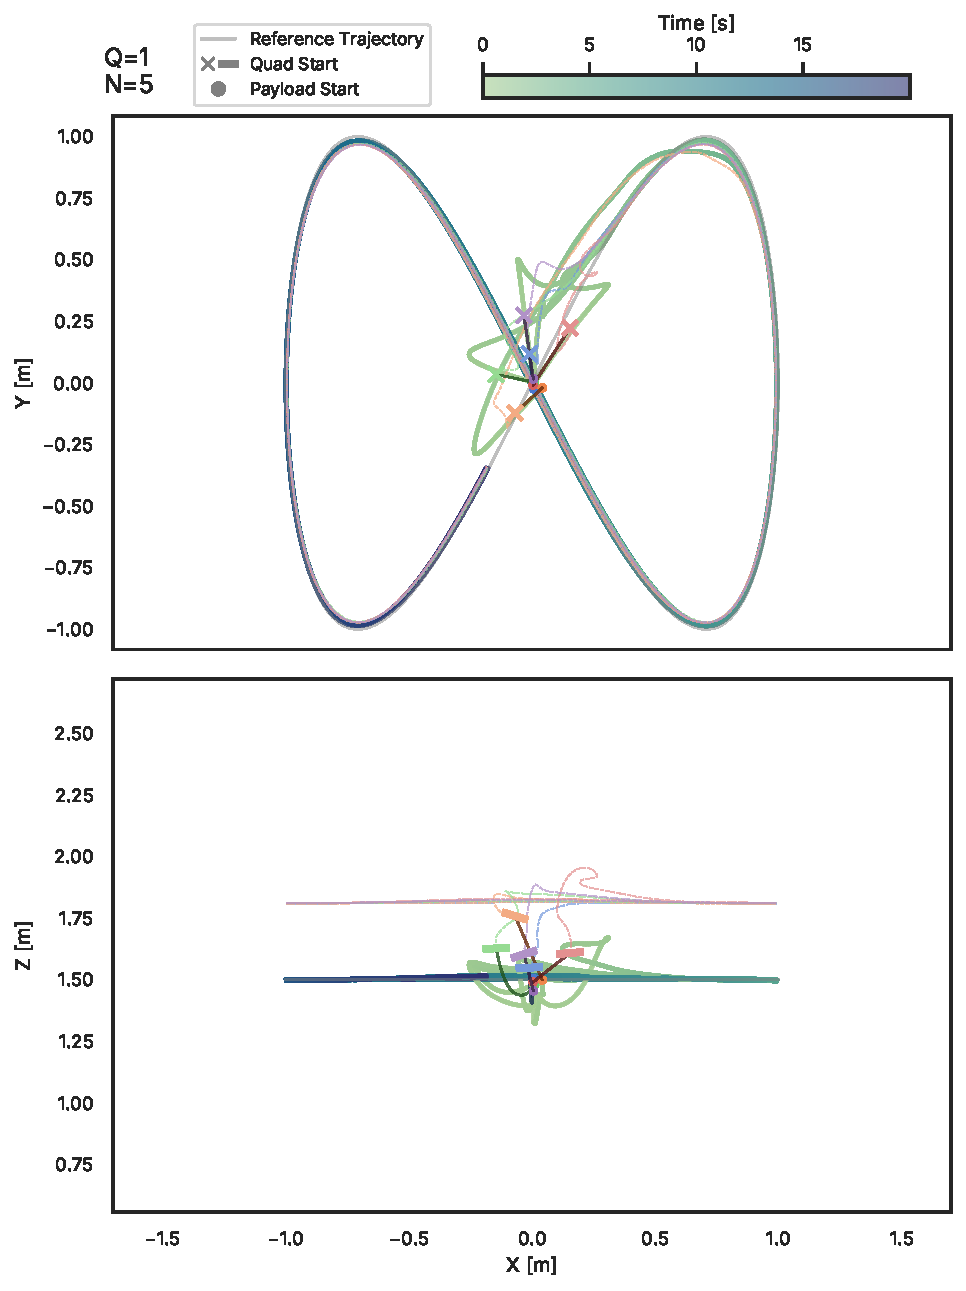
\includegraphics[width=\textwidth]{experiments/one_eight.pdf}
    \caption{Figure-eight trajectory tracking for one quadrotor with payload.The top plot is top-down  (xy) view, while the bottom one is side view (xz). The figure shows N=5 runs. The position is initialized near the target with random quadrotor states. The quadrotor successfully follows the figure-eight path while stabilizing the payload.}
    \label{fig:one_eight}
\end{figure}

\section{Multi-Quadrotor Payload Transport}
We extend the evaluation to cooperative transport tasks involving teams of two and three quadrotors to show learned coordinated behavior. The simulation configuration and scenarios are setup similarly to the single-quadrotor case, with the payload always initialized at $(0 0 1.5)$ m and the quadrotors positioned randomly in a half-sphere around it as described in \ref{sec:reset}. The policies are trained specifically for the specific number of quadrotors in the team. For three quadrotors we increase the payload mass to 20g to ensure that the payload is heavy enough to require cooperation. The policies are trained using the \gls{ippo} algorithm with the same hyperparameters as in the single-quadrotor case.
\subsection{Two Quadrotors}
We first evaluate the learned policy on the two-quadrotor case, testing both harsh condition recovery and trajectory tracking on a figure-eight path. We run each of them with the policy trained specifically for the two quadrotor with payload scenario. The results are shown in Figure \ref{fig:payload_error_over_time_two}, Figure \ref{fig:two_recovery} and Figure \ref{fig:two_eight}.

Figure \ref{fig:two_recovery} shows some example runs of the recovery task, where the quadrotors and payload are initialized in random states and have to stabilize the payload at the target position. The runs labeled 0 and 1 show successful takeoff. 4 and 3 shaow stabilizatition of swinging payload. 4 in specific shows a very harsh tilt orientation of the quad that is recovered from. 3 to 7 are all initialized with slack cables. the paylaod is stabilized at the target within 2 seconds, moving at speeds of up to 1.5 m/s. The quadrotors then stabilize the payload at the target position without oscillations or overshoot.
We also evaluate this in figure \ref{fig:payload_error_over_time_two}, where we statistically evaluate 1000 recovery runs from harsh conditions. The termination histogram shows that 81\% of harsh initial conditions are recovered successfully, while the remaining terminate mostly in the beginning due to very harsh initialization. The position error over time also shows that we recover from distances of up to 1m in roughly 2s. It also shows that all runs stabily hove at the target for over 5s after they reaching it. Some off the failed runs struggle to recover and get stuck in an oscillation leading to termination. This is due to very harsh initlalization, leading to the quadrotors running into each other right after initialization. This can be improved by better initialization of the quadrotors and payload, which is discussed in section \ref{sec:reset}.

To show that the position tracking capabilities generalize to a moving setpoint we evaluate on a precomputed figure eight trajectory. We use the same setup as with the single quad case. We show the result in figure \ref{fig:two_eight}. The figure shows the path of 5 runs randomly initialized around the start point of the trajectory, with the quads in suboptimal states. The figure shows how the quads very fast manage to stabilize themselfs and then continue after around 3s to very follow the trajectory. The tracking is a bit less accurate then the single quad case, but still shows good performance. Eventhough all quads are initialized with slightly different thrust ranges they all manage to accurately track the correct height of the trajectory. We might further improve the tracking performance by explicitly training on trajectory following and adding multiple trajectory points or velocity states as shown in previous work and also adding the velocity state of the other quadrotors additionally to the relative position to the observation space.
\begin{figure}[ht]
    \centering
    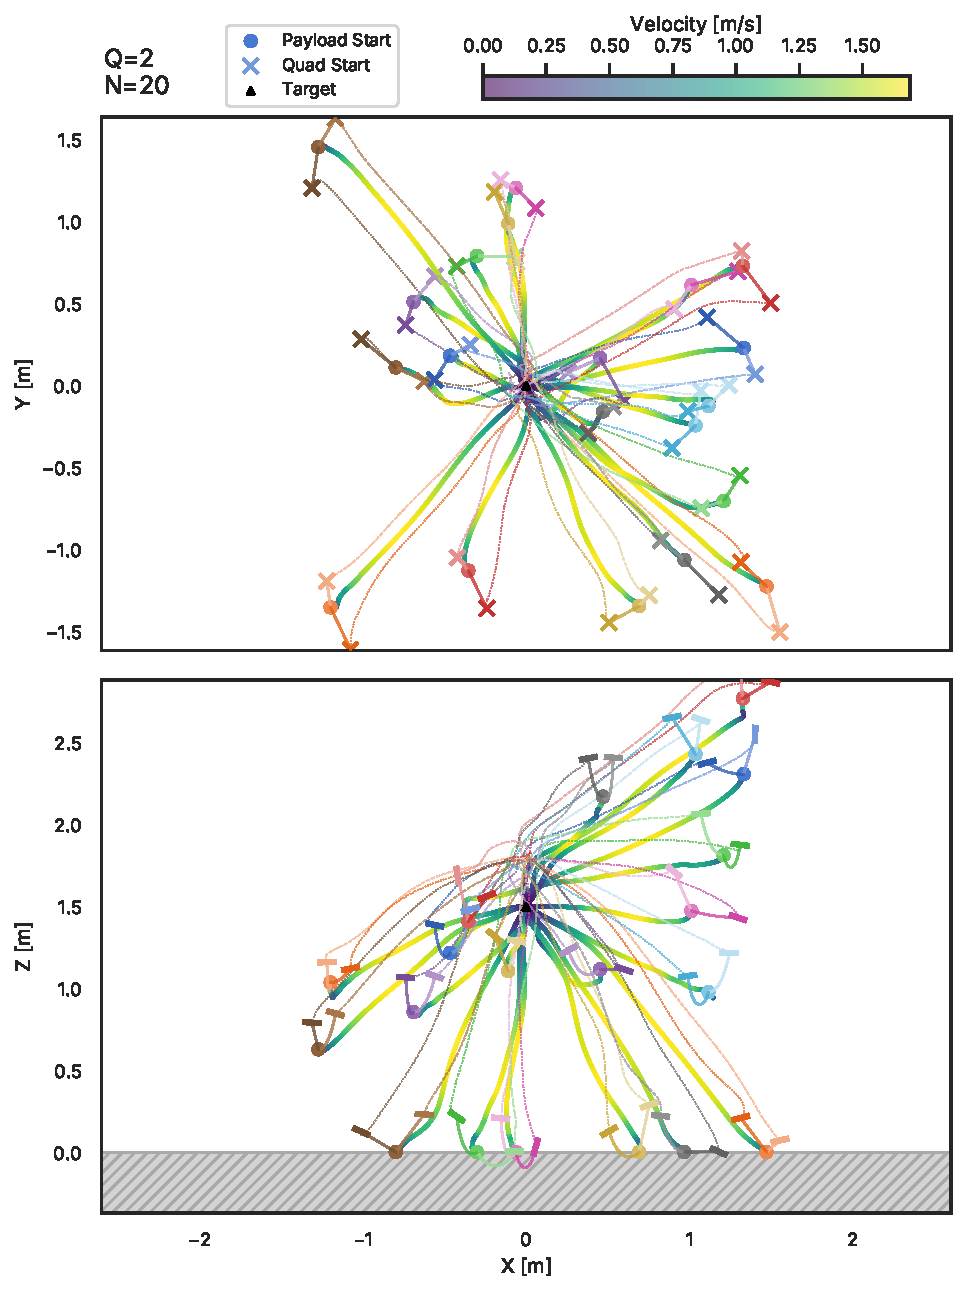
\includegraphics[width=\textwidth]{experiments/two_recovery.pdf}
    \caption{Recovery of two quadrotors with payload from harsh conditions. The top plot is top-down  (xy) view, while the bottom one is side view (xz).
    The figure shows N=8 runs. The position of payload and quadrotors is initialized randomly and the goal is to recover to the target and stabilize. The quadrotor successfully stabilizes the payload within 2 seconds. The initial states of the quadrotor and payload are marked and labeled with their run id. The cables are drawn to represent their mode and cable lengt, slackness in the cable being shown as a curve.}
    \label{fig:two_recovery}
\end{figure}
\begin{figure}[ht]
    \centering
    
    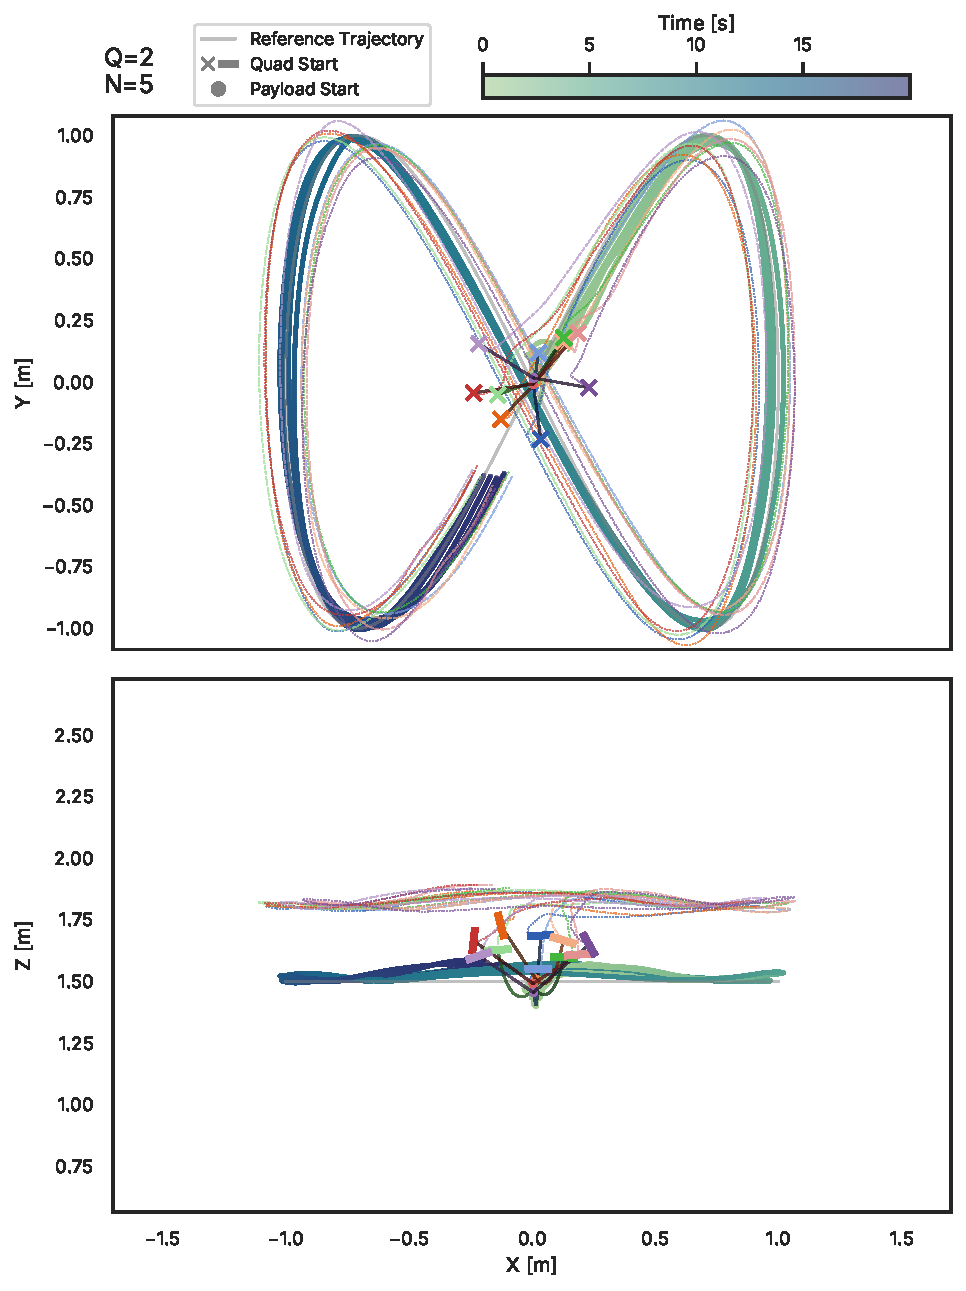
\includegraphics[width=\textwidth]{experiments/two_eight.pdf}
    \caption{Figure-eight trajectory tracking for two quadrotors with payload.The top plot is top-down  (xy) view, while the bottom one is side view (xz). The figure shows N=5 runs. The position is initialized near the target with random quadrotor states. The quadrotor successfully follows the figure-eight path while stabilizing the payload.}
    \label{fig:two_eight}
\end{figure}

% optional
\section{Comparison with classic control}
Compare with prev paper method \autocite{Wahba2024}
\begin{itemize}
    \item Plots Traj: Trajectory following 3d, error over time for batch
    \item Plots Disturbance: Trajectory following with disturbance, error over time for batch
    \item Plots ground start: Trajectory following with disturbance, error over time for batch
\end{itemize} 
\section{Sim-to-Real Transfer}
\begin{itemize}
    \item one and three quads
    \item Plots Traj: Trajectory following 3d,  error over time 
    \item Plots Disturbance: Position holding with disturbance
\end{itemize}

\section{Generalization}
Does it generalize to different payloads?
